\documentclass[aspectratio=169]{beamer}
\setbeamertemplate{navigation symbols}{}
\usepackage{color, amsmath, comment, subfigure}
\usepackage{url}
\usepackage{ulem}

\usepackage{hyperref}
\hypersetup{
    colorlinks=true,
    linkcolor=blue,
    filecolor=magenta,      
    urlcolor=cyan,
}

%%%%%%%%%%%%%%%%%%%%%%%%%%
\title[]{Class slides for Tuesday, October 20:\\Weather, Lorenz attractor}
\author[]{Matthew J. Salganik}
\institute[]{}
\date[]{COS 597E/SOC 555 Limits to prediction\\Fall 2020, Princeton University}

\begin{document}
%%%%%%%%%%%%%%%%%%%%%%%%%%%
\frame{\titlepage}
%%%%%%%%%%%%%%%%%%%%%%%%%%%
\begin{frame}

``My other classes make me feel smarter and this class makes me feel dumber.''\\
- An undergraduate at Columbia about 10 years ago.

\pause
\vfill
\begin{itemize}
\item classes that help you answer questions
\item classes that help you ask questions
\end{itemize}

\end{frame}
%%%%%%%%%%%%%%%%%%%%%%%%%%%%
\begin{frame}

Lorenz's work on deterministic chaos ``profoundly influenced a wide range of basic sciences and brought about one of the most dramatic changes in mankind's view of nature since Sir Isaac Newton.''\\
 
-1991 Kyoto Prize for basic sciences in the field of earth and planetary sciences.

\end{frame}
%%%%%%%%%%%%%%%%%%%%%%%%%%%%
\begin{frame}

\Large{
Deterministic and unpredictable 
}

\end{frame}
%%%%%%%%%%%%%%%%%%%%%%%%%%%%
\begin{frame}
\frametitle{}

\begin{center}
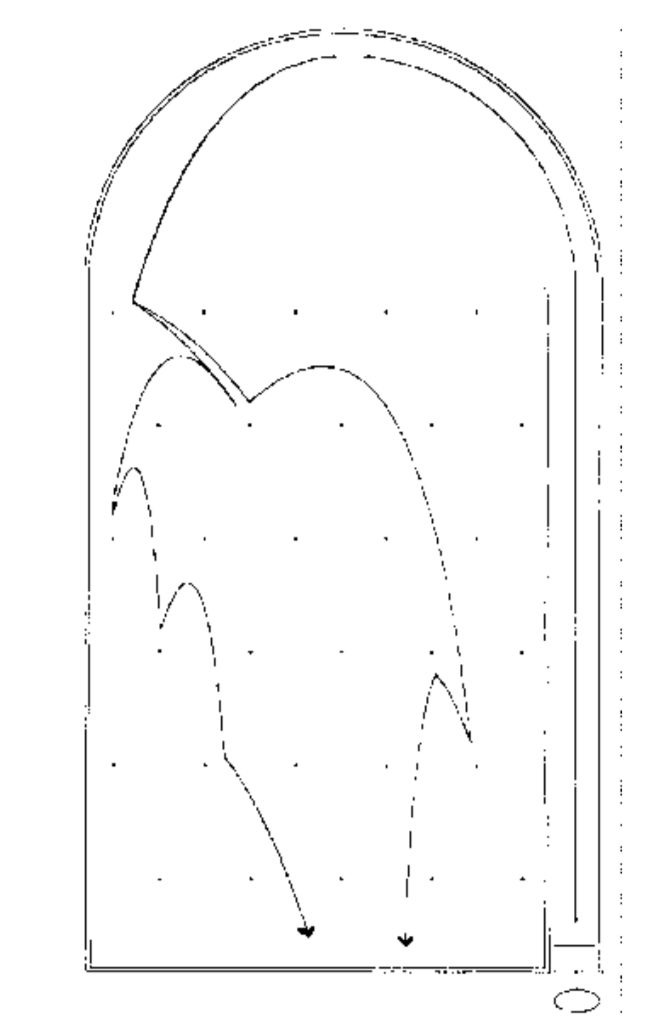
\includegraphics[height = 0.9\textheight]{figures/lorenz_essence_1993_fig1}
\end{center}

\end{frame}
%%%%%%%%%%%%%%%%%%%%%%%%%%%%%
\begin{frame}
\frametitle{}

\begin{center}
\only<1>{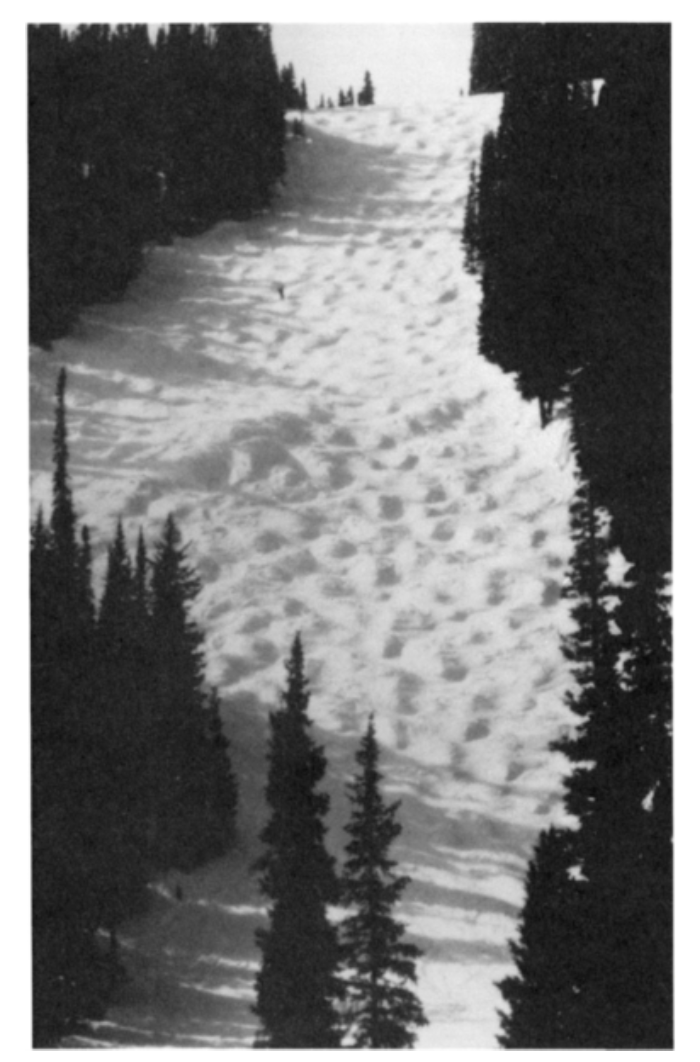
\includegraphics[height = 0.9\textheight]{figures/lorenz_essence_1993_fig5}}%
\only<2>{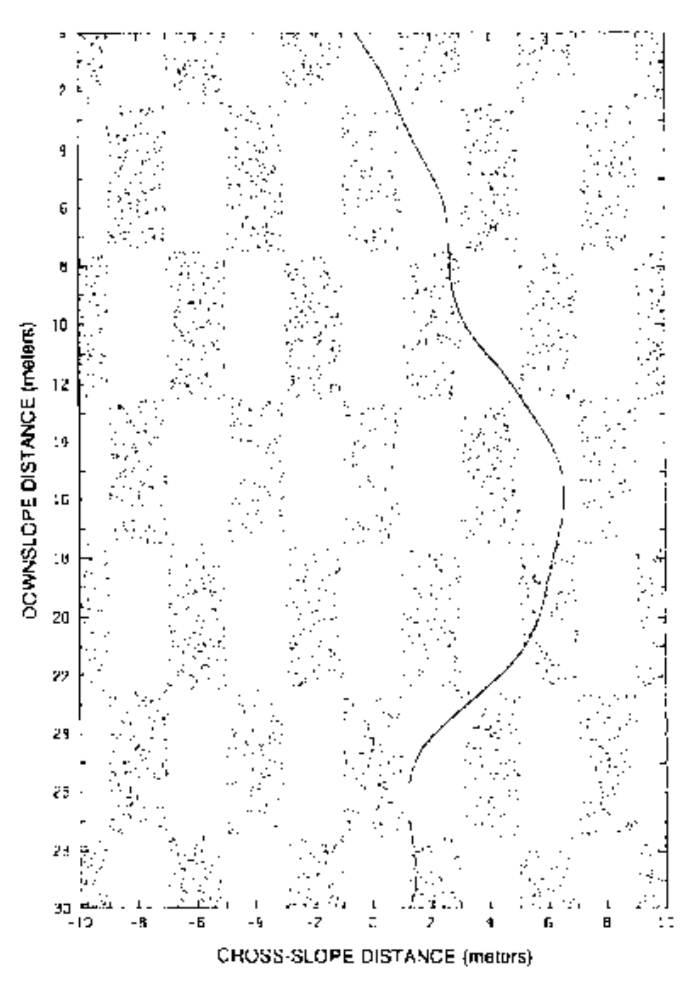
\includegraphics[height = 0.9\textheight]{figures/lorenz_essence_1993_fig6}}%
\only<3>{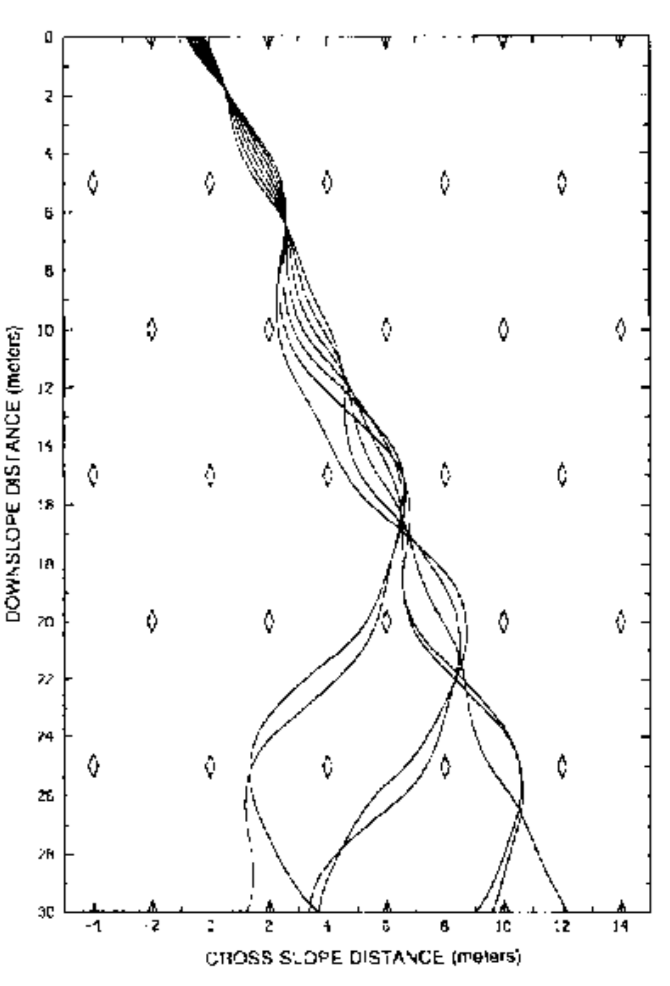
\includegraphics[height = 0.9\textheight]{figures/lorenz_essence_1993_fig7}}%
\only<4>{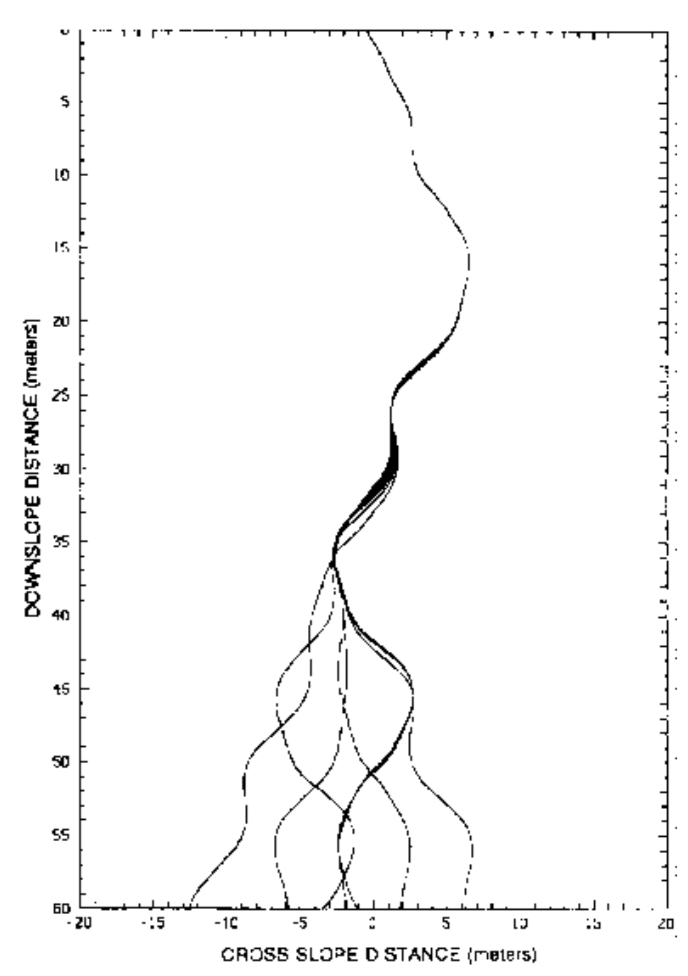
\includegraphics[height = 0.9\textheight]{figures/lorenz_essence_1993_fig8}}%
\end{center}

\end{frame}
%%%%%%%%%%%%%%%%%%%%%%%%%%%%%
\begin{frame}
\frametitle{}

Sensitive dependence on initial conditions: two nearly identical initial conditions diverge until they bear not more resemblance than two states chosen randomly

\end{frame}
%%%%%%%%%%%%%%%%%%%%%%%%%%%%%
\begin{frame}

\begin{center}
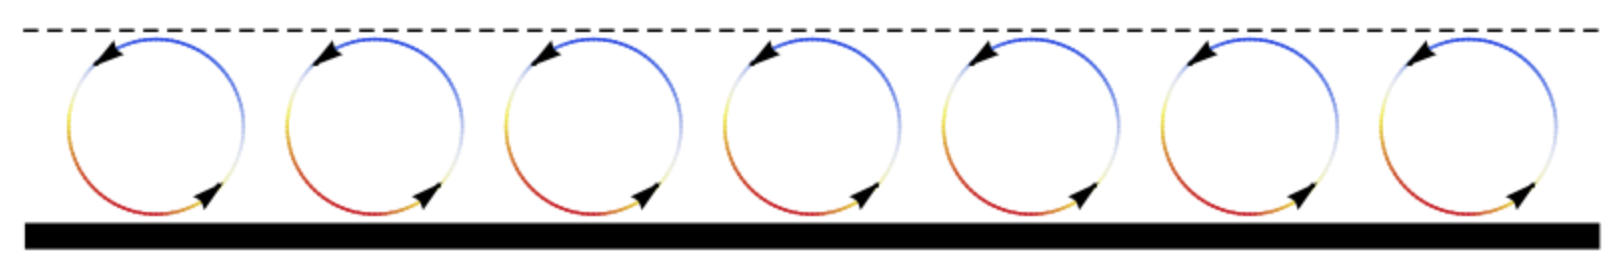
\includegraphics[width = 0.9\textwidth]{figures/lorenz_rolls}
\end{center}

\begin{itemize}
\item x: the rate of convective motion - i.e. how fast the rolls are rotating,
\item y: the temperature difference between the ascending and descending currents
\item z: the distortion (from linearity) of the vertical temperature profile.
\end{itemize}

\vfill
\tiny{\url{https://marksmath.org/visualization/LorenzExperiment/}}

\end{frame}
%%%%%%%%%%%%%%%%%%%%%%%%%%%%%
\begin{frame}

\begin{align*}
  x' &= \sigma(y-x) \\
  y' &= x(\rho-z)-y \\
  z' &= xy-\beta z
\end{align*}
\begin{center}
$\sigma = 10, \rho = 28,  \beta = 8/3$ 
\end{center}

\begin{center}
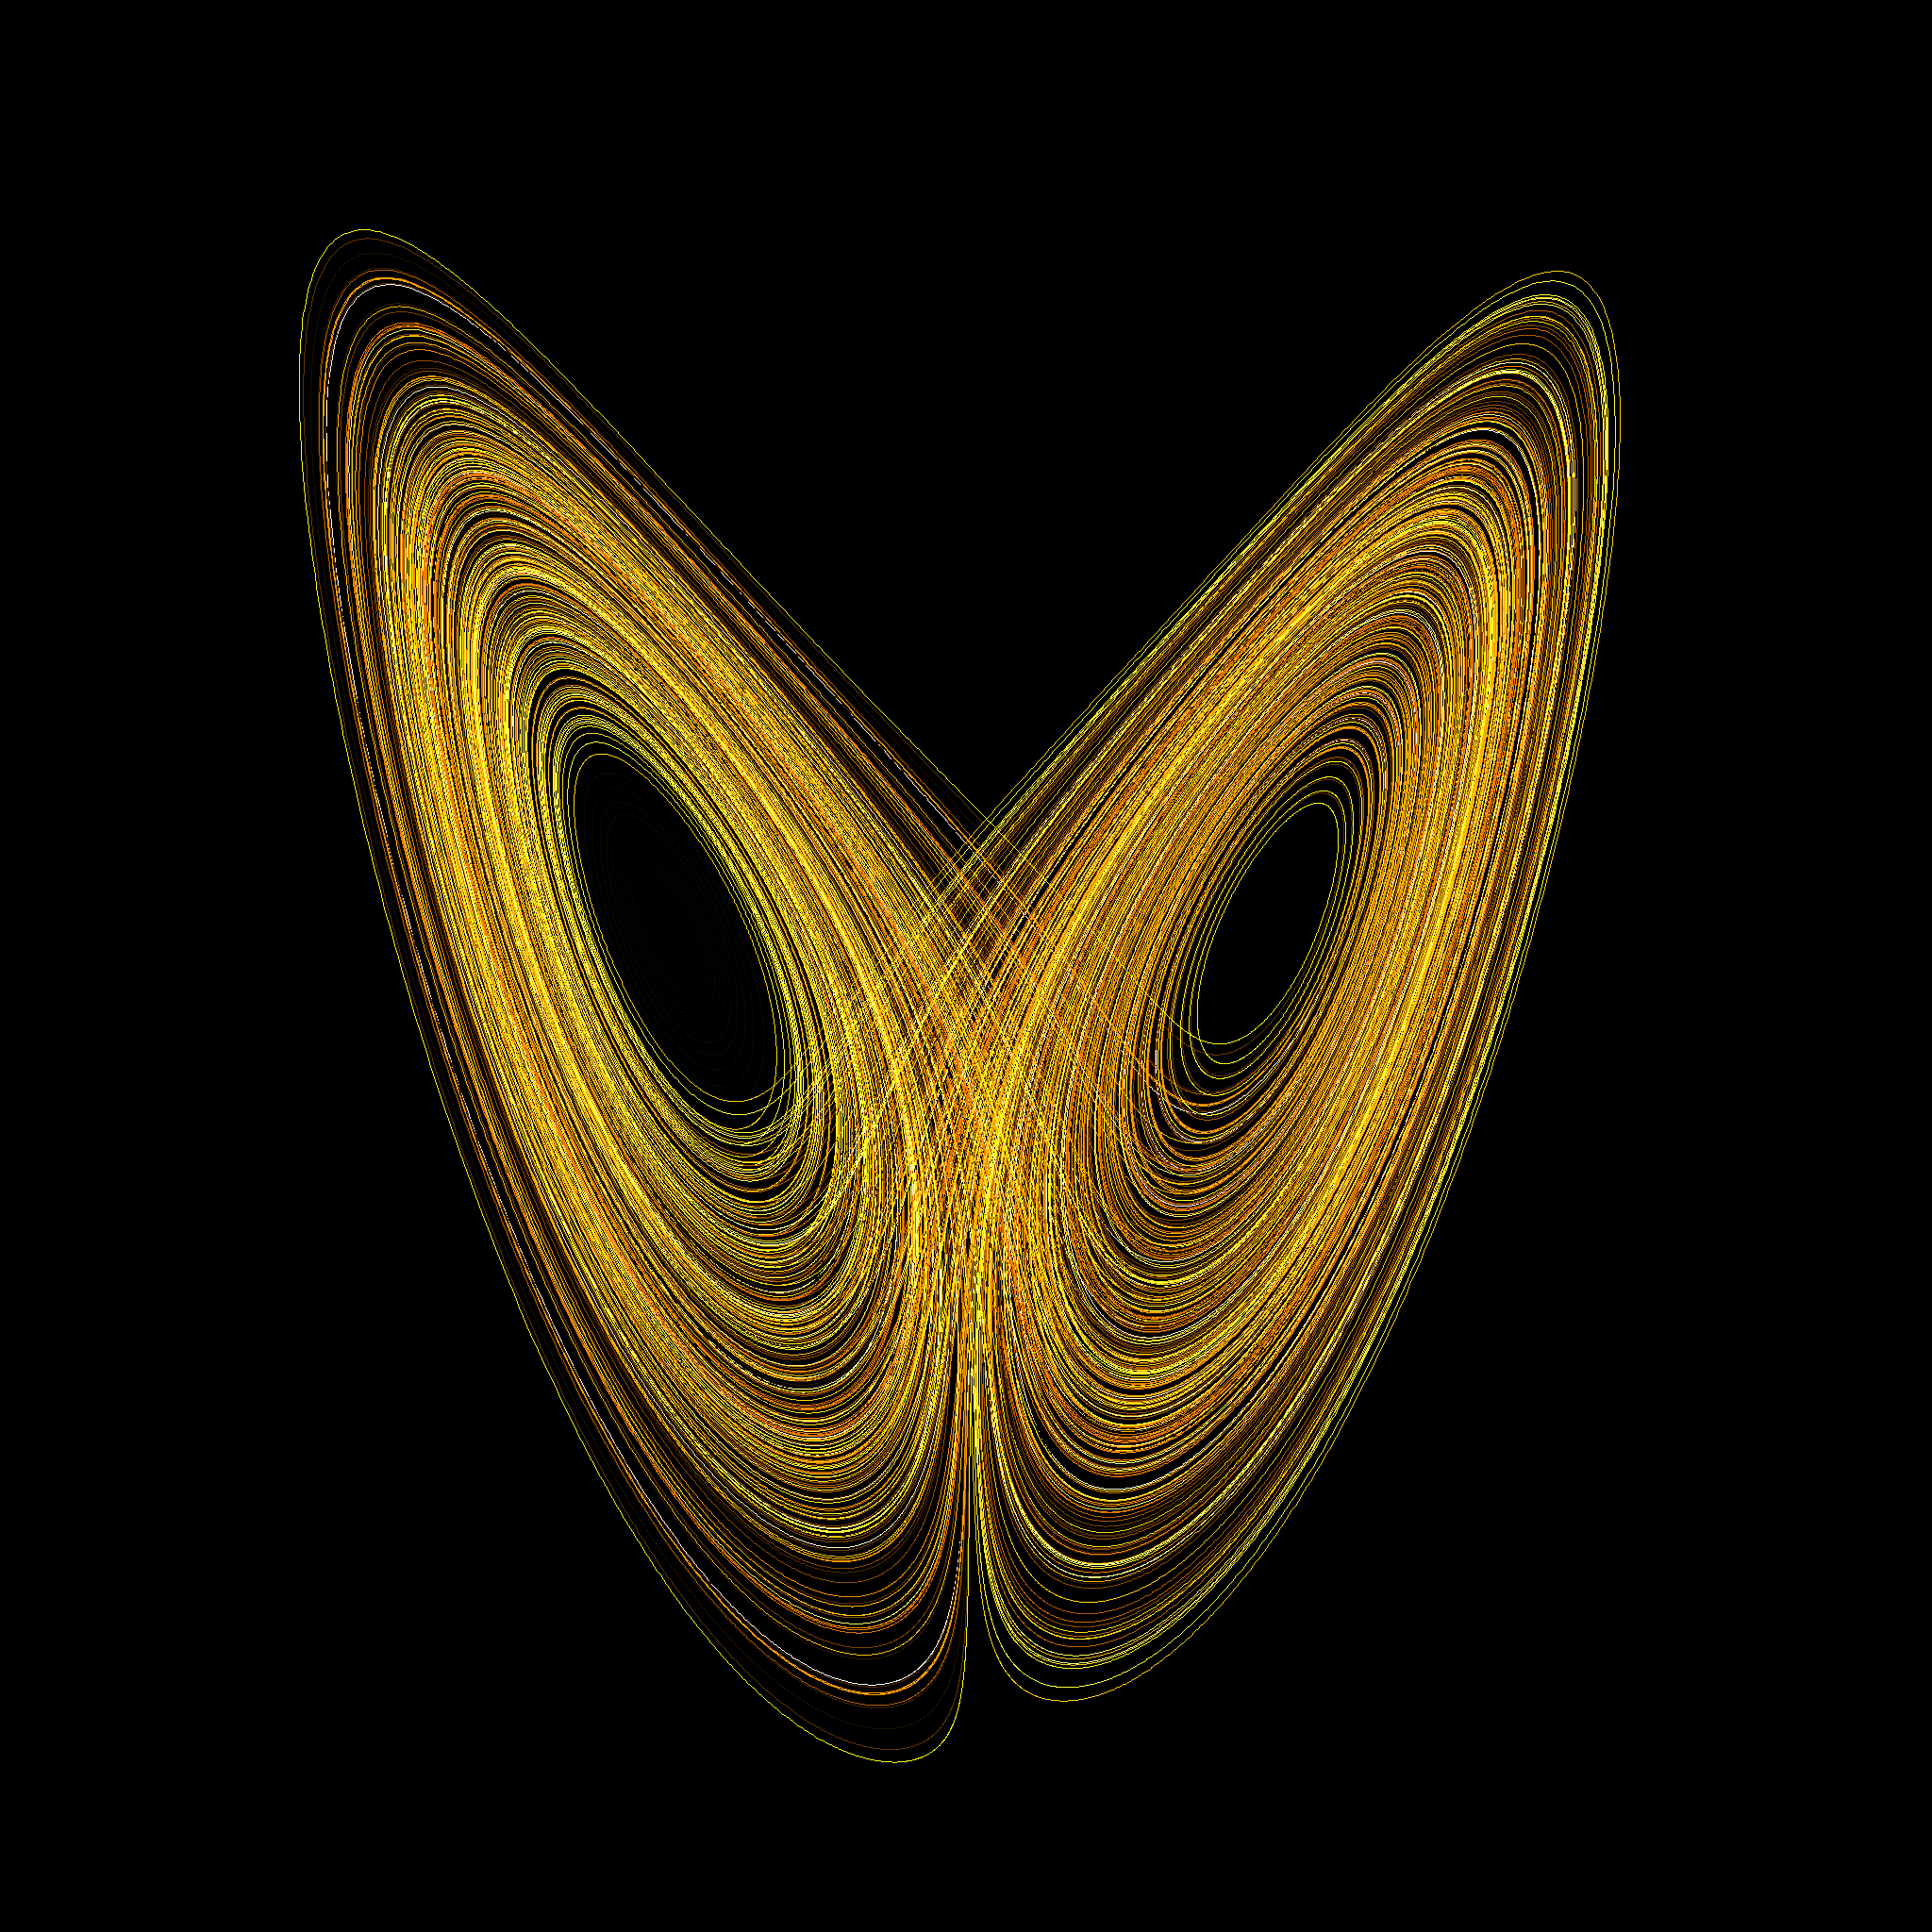
\includegraphics[width = 0.3\textwidth]{figures/Lorenz_system_r28_s10_b2-6666}
\end{center}

\vfill
\tiny{\url{https://commons.wikimedia.org/wiki/File:Lorenz_system_r28_s10_b2-6666.png}}
\end{frame}
%%%%%%%%%%%%%%%%%%%%%%%%%%%%%
\begin{frame}

DEMO: \url{https://marksmath.org/visualization/LorenzExperiment/}

\end{frame}
%%%%%%%%%%%%%%%%%%%%%%%%%%%%%
\begin{frame}

\Large{
BREAK INTO GROUPS
}

\end{frame}
%%%%%%%%%%%%%%%%%%%%%%%%%%%
\begin{frame}

If we reduce measurement error how much time does that buy us? \pause
Not much

\end{frame}
%%%%%%%%%%%%%%%%%%%%%%%%%%%
\begin{frame}

Simulation results, switch to R

\end{frame}
%%%%%%%%%%%%%%%%%%%%%%%%%%%
\begin{frame}

\begin{center}
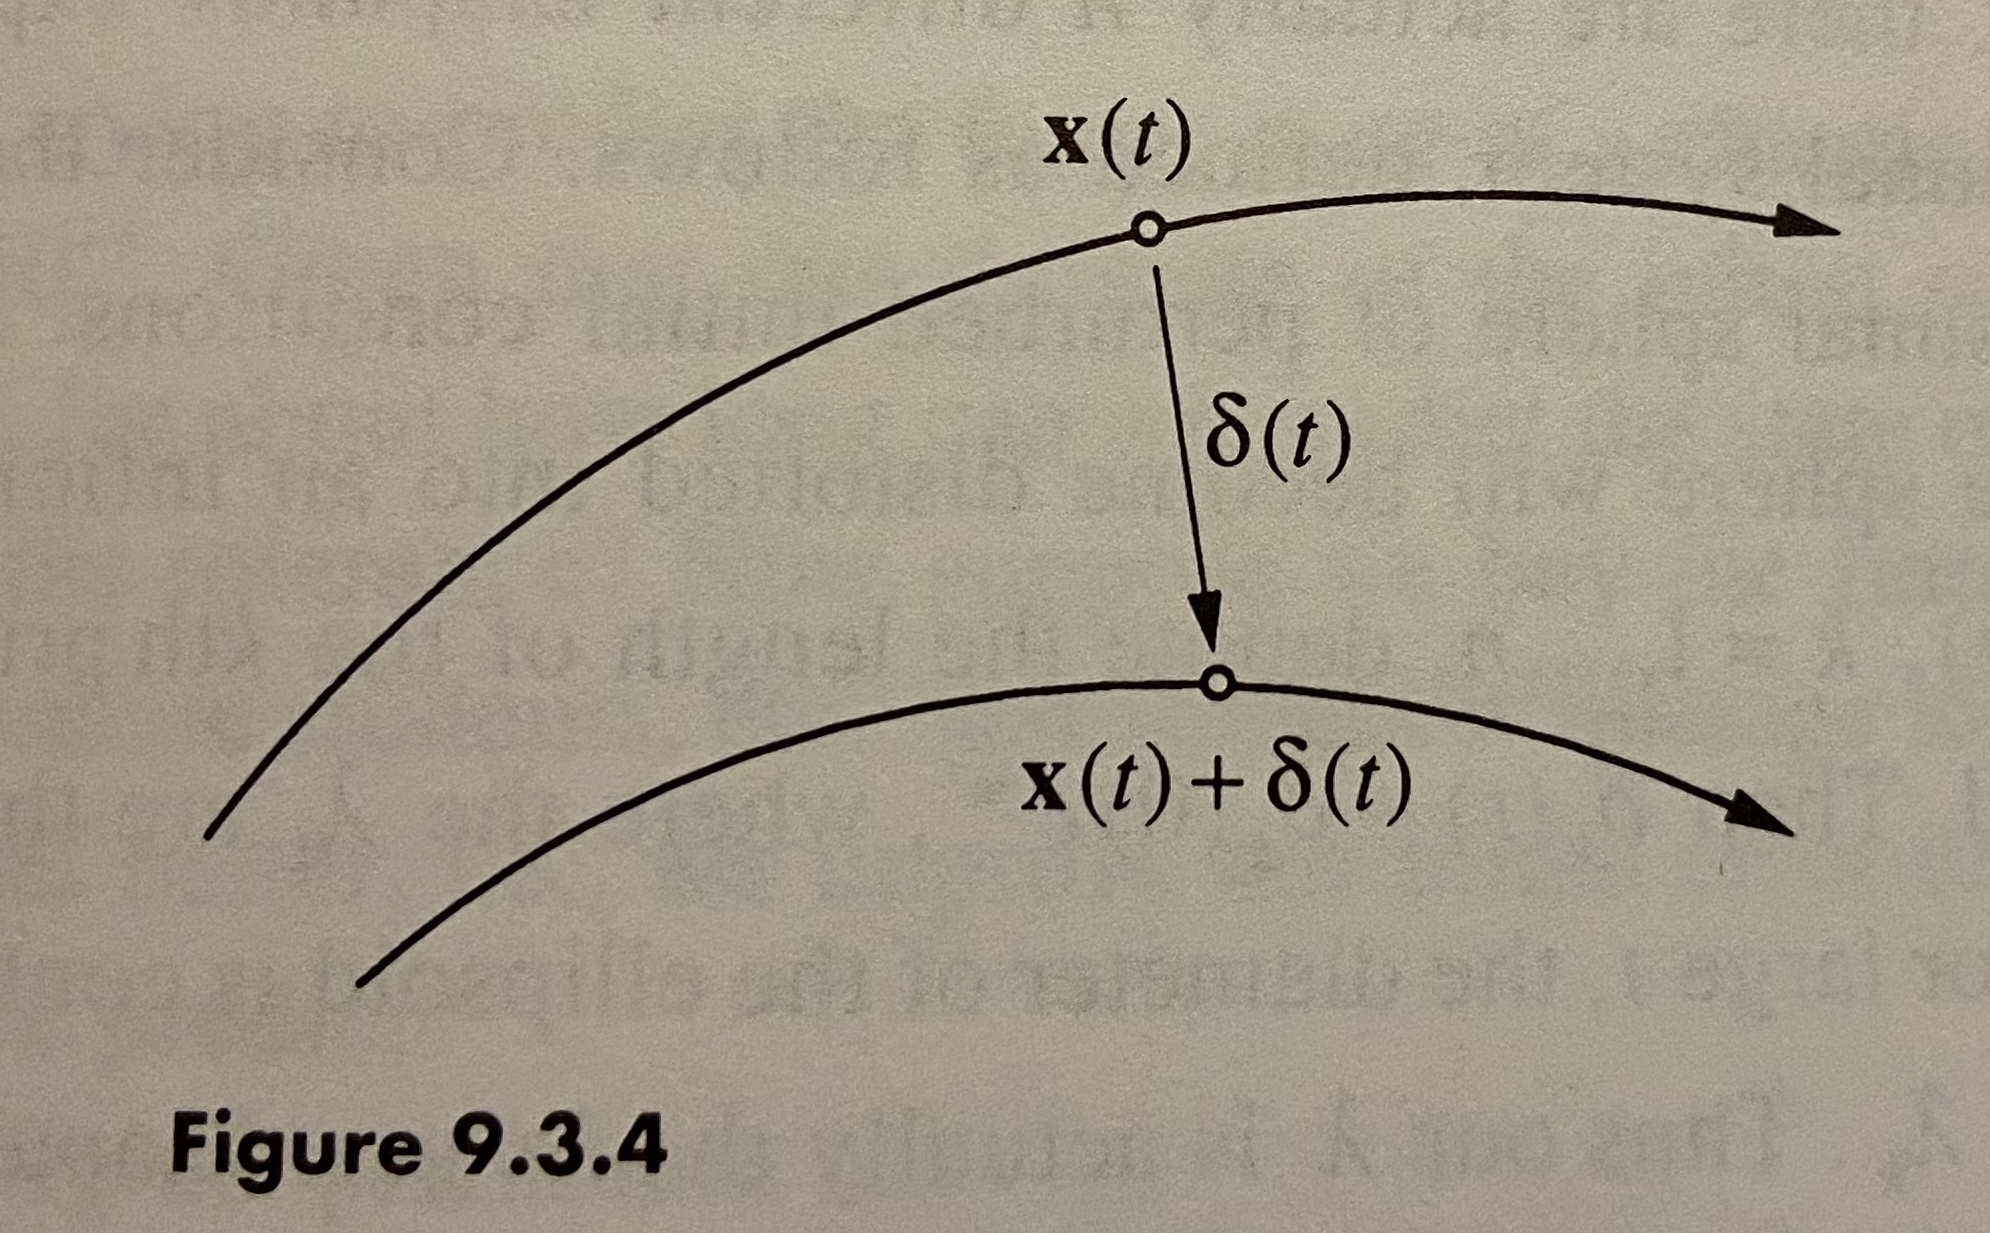
\includegraphics[width = 0.5\textwidth]{figures/strogatz_nonlinear_1994_fig9_3_4}
\end{center}

\pause

It turns out that:\\
$ \underbrace{\left\Vert  \delta(t) \right\Vert}_{\text{divergence at time $t$}} \sim  \underbrace{\left\Vert \delta_0 \right\Vert}_{\text{initial divergence}}\underbrace{e^{\lambda t}}_{\text{rate of growth}}$

where:\\
$\lambda$ is called the Liapunov exponent and it varies from system to system
\vfill
Strogatz (1994), Sec 9.3
\end{frame}
%%%%%%%%%%%%%%%%%%%%%%%%%%%
\begin{frame}

Let $a$ be a measure of tolerance and $t_{horizon}$ be the time that the discrepancy between two trajectories exceeds our tolerance, it turns out that\\

$t_{horizon} \sim O \left( \frac{1}{\lambda} ln \frac{a}{\left\Vert \delta_0 \right\Vert} \right)$
 
Because of the logarithmic dependence on $\left\Vert \delta_0 \right\Vert$, we need order of magnitude decreases in $\left\Vert \delta_0 \right\Vert$ in order to produce one extra multiple of $\frac{1}{\lambda}$.  For Lorenz system $\lambda \approx 0.9$.  
 
\vfill
Strogatz (1994), Sec 9.3
\end{frame}
%%%%%%%%%%%%%%%%%%%%%%%%%%%%
\begin{frame}

\begin{center}
\Large{
Compare and contrast to other work
}
\end{center}

\end{frame}
%%%%%%%%%%%%%%%%%%%%%%%%%%%%
\begin{frame}

These systems seem to be unpredictable in some ways and predictable in other ways:
\url{https://www.youtube.com/watch?v=6YDHBFVIvIs}

\end{frame}
%%%%%%%%%%%%%%%%%%%%%%%%%%%%
\begin{frame}

These systems seem to be unpredictable in some ways and predictable in other ways \pause
\begin{center}
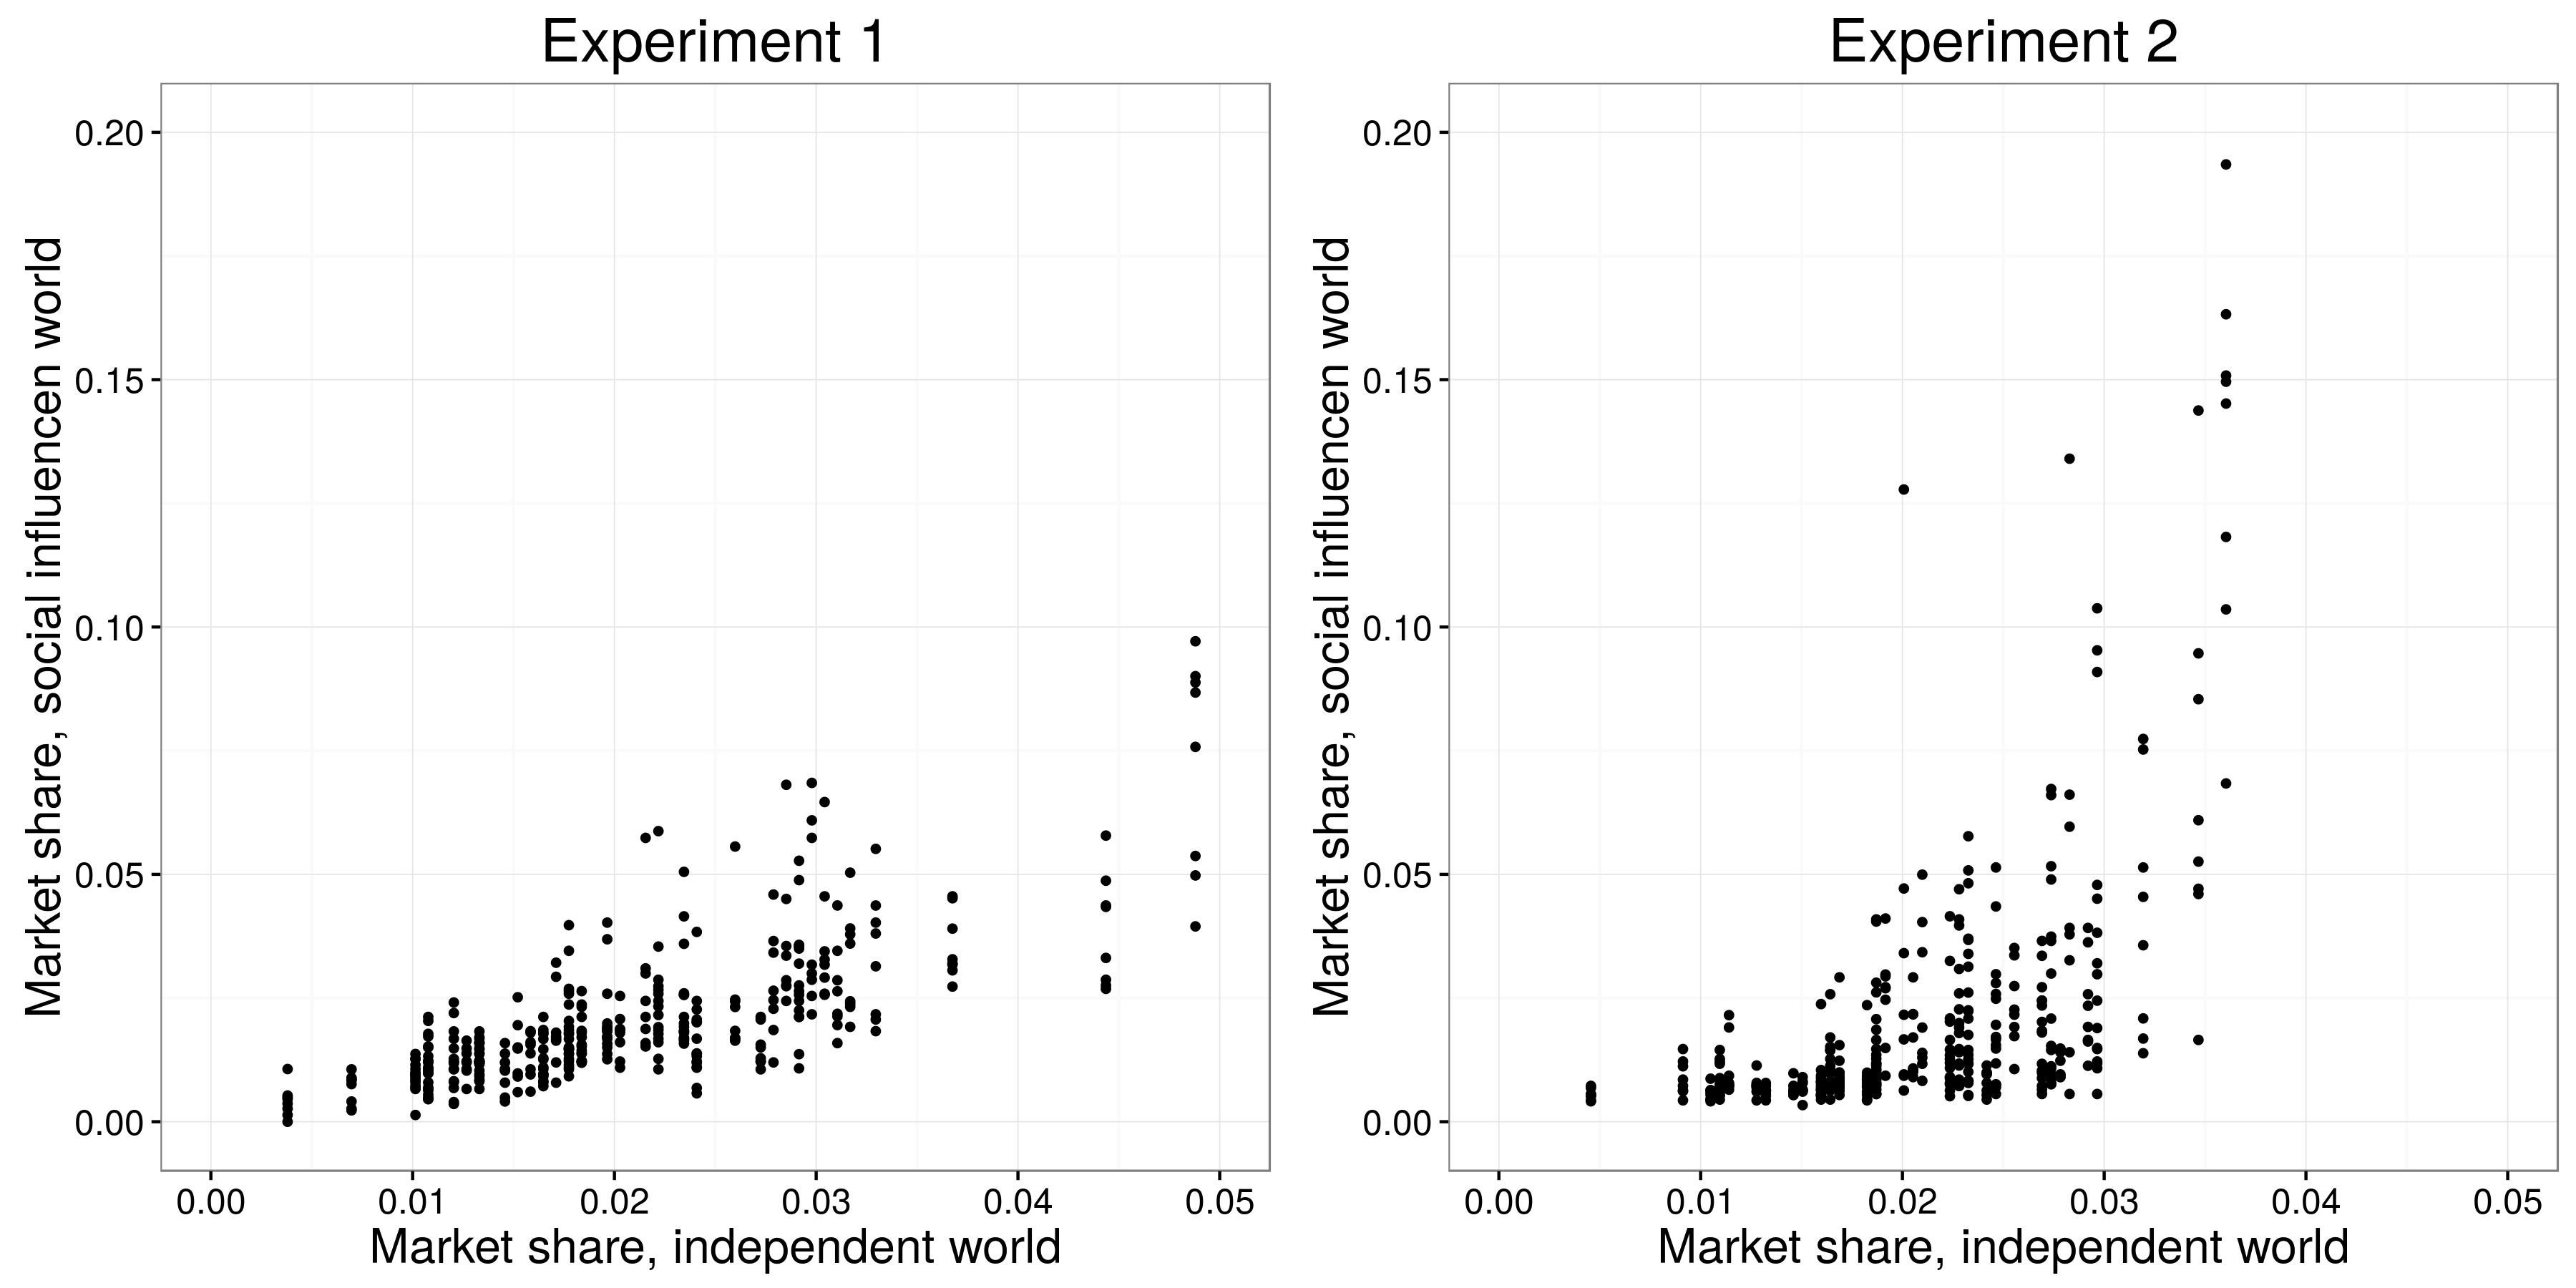
\includegraphics[width = 0.9\textwidth]{figures/bitbybit4-23_salganik_experimental_2006_fig3ac}
\end{center}

\end{frame}
%%%%%%%%%%%%%%%%%%%%%%%%%%%%
\begin{frame}

\begin{center}
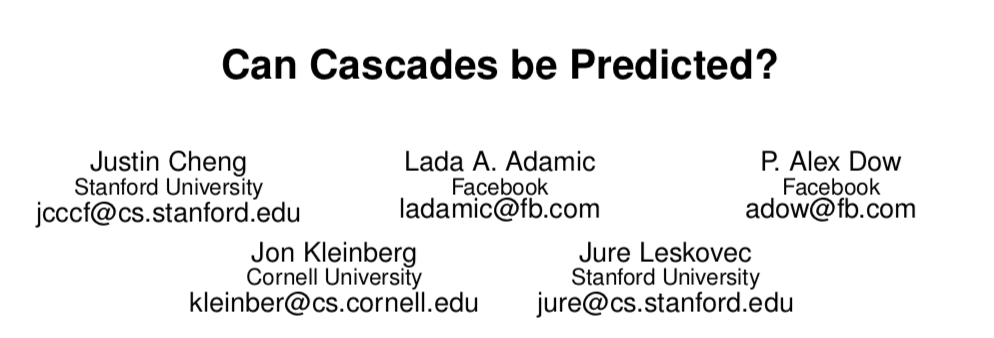
\includegraphics[width = 0.9\textwidth]{figures/cheng_can_2014_title}
\end{center}

\vfill
Deals with time in a different way 
\end{frame}
%%%%%%%%%%%%%%%%%%%%%%%%%%%%
\begin{frame}

\begin{center}
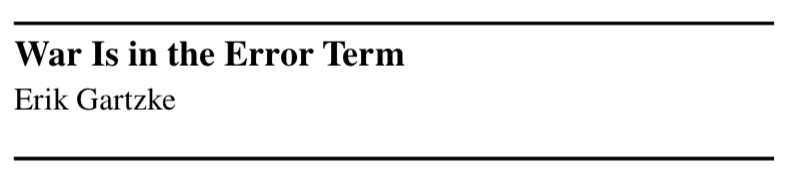
\includegraphics[width = 0.9\textwidth]{figures/gartzke_war_1999_title}
\end{center}

\vfill
Lorenz system more clearly shows a limit to prediction in a model that seems reasonable (to me)

\end{frame}
%%%%%%%%%%%%%%%%%%%%%%%%%%%%%%%%%
\begin{frame}

Showing sensitive dependence seems like a rigorous way to show a limit to prediction, but it seems detached from how we talked about measuring predictability last class (e.g., $R^2$, $MSE$, etc) and how we talk about unpredictability (e.g., Bayes error rate)

\end{frame}
%%%%%%%%%%%%%%%%%%%%%%%%%%%%%%%%%
\begin{frame}

\begin{columns}[c]
  \column{.5\textwidth}
  \begin{center}
  Data generating process in statistics/machine learning\\
  $y = f(x) + \epsilon$
  \end{center}
    \column{.5\textwidth} \pause
   \begin{center}
  Data generating process in dynamical systems\\
\begin{align*}
  x' &= \sigma(y-x) \\
  y' &= x(\rho-z)-y \\
  z' &= xy-\beta z
\end{align*}
\begin{center}
$\sigma = 10, \rho = 28,  \beta = 8/3$ 
\end{center}
    \end{center}
\end{columns}

\vfill
Thinking back to Breiman, I wonder if these are different cultures with different approaches to predictability

\end{frame}
%%%%%%%%%%%%%%%%%%%%%%%%%%%%%%%%%
\begin{frame}

\Large{
\only<1>{Can deep learning predict chaotic systems?}
\only<2>{Can \sout{deep learning} reservoir computing predict chaotic systems?}
}

\end{frame}
%%%%%%%%%%%%%%%%%%%%%%%%%%
\begin{frame}

\begin{center}
\only<1>{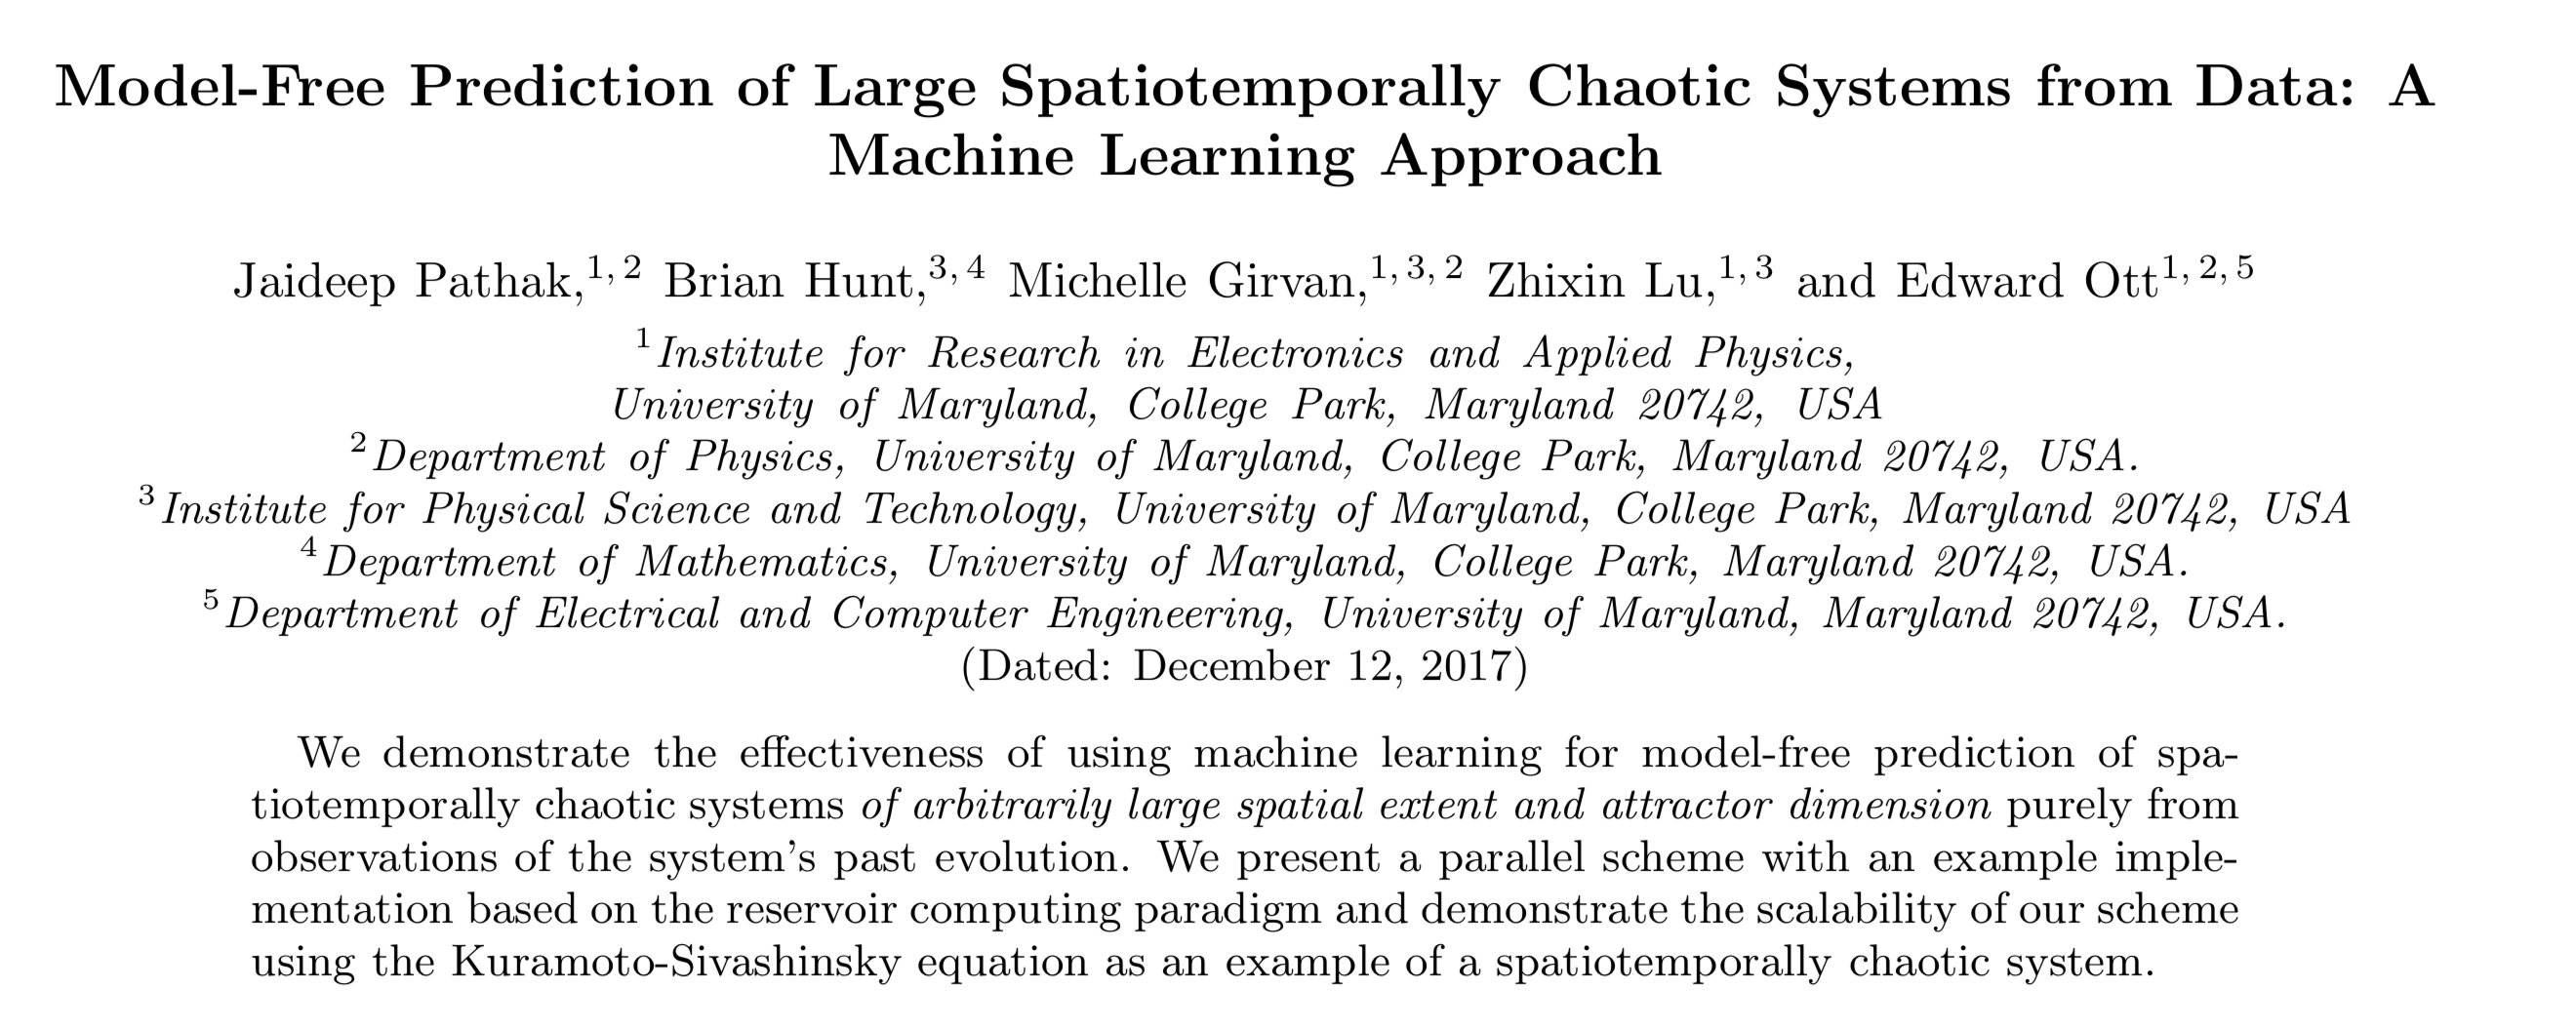
\includegraphics[width = 0.9\textwidth]{figures/pathak_model-free_2018_title_abstract}}
\only<2>{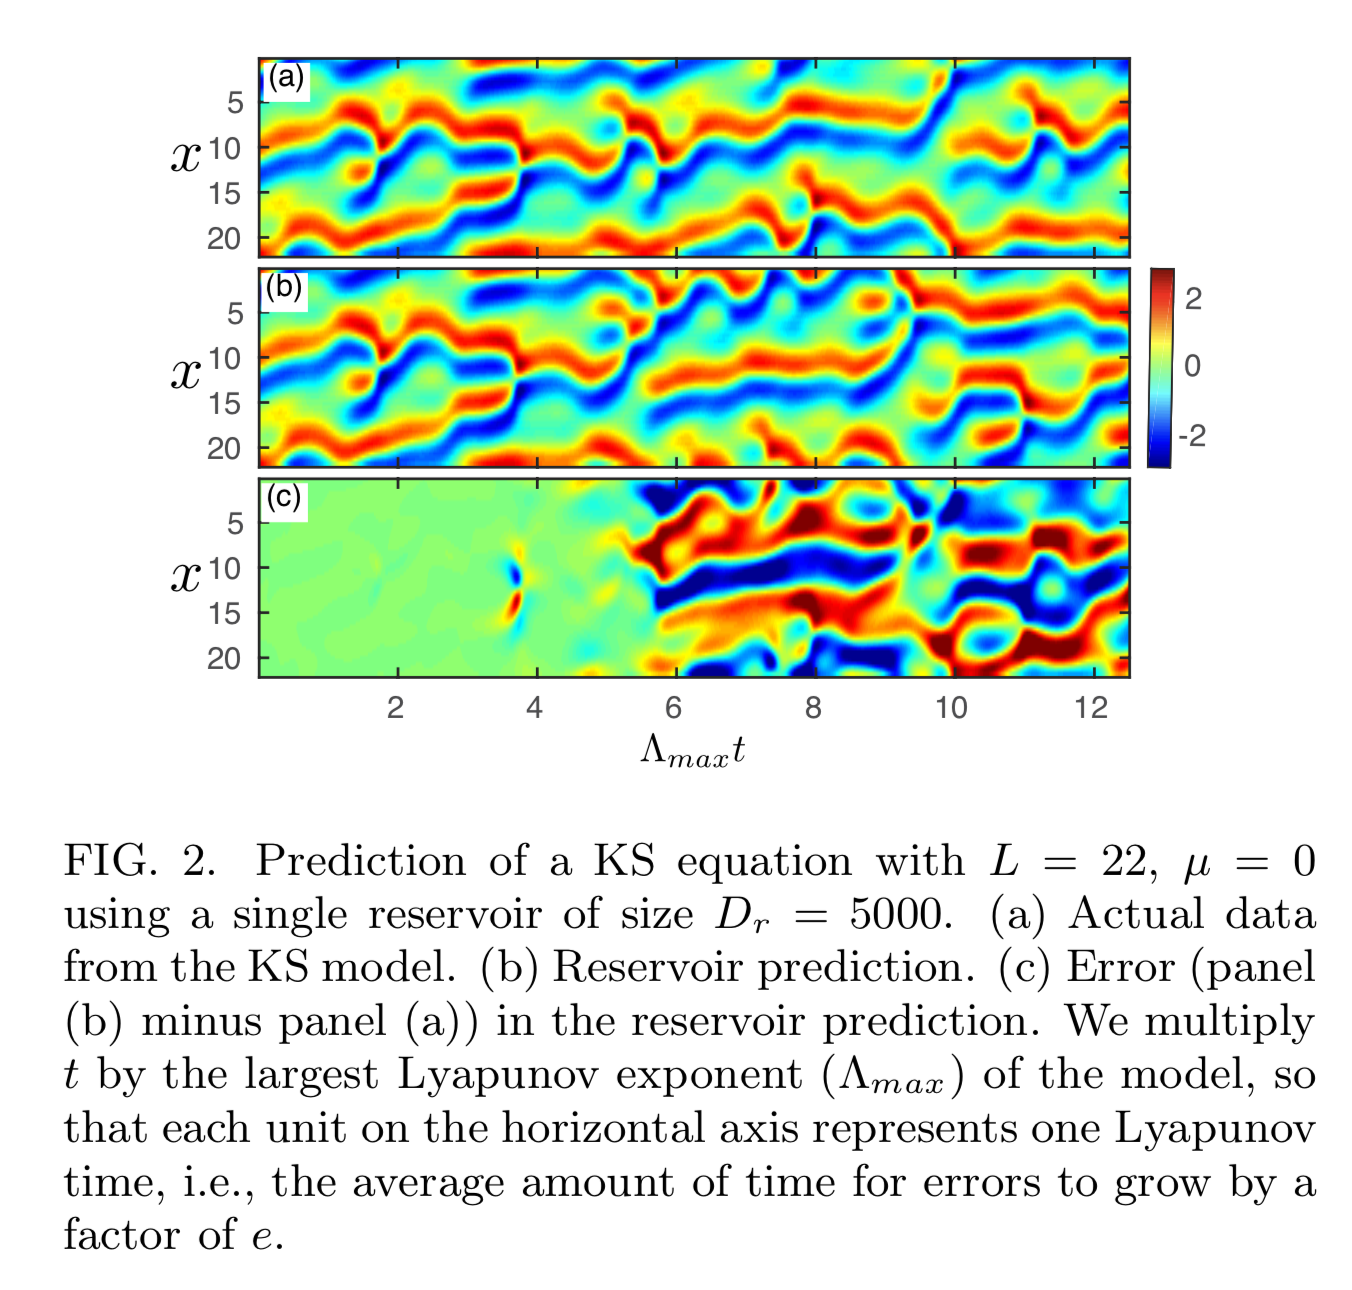
\includegraphics[width = 0.6\textwidth]{figures/pathak_model-free_2018_fig2}}
\only<3>{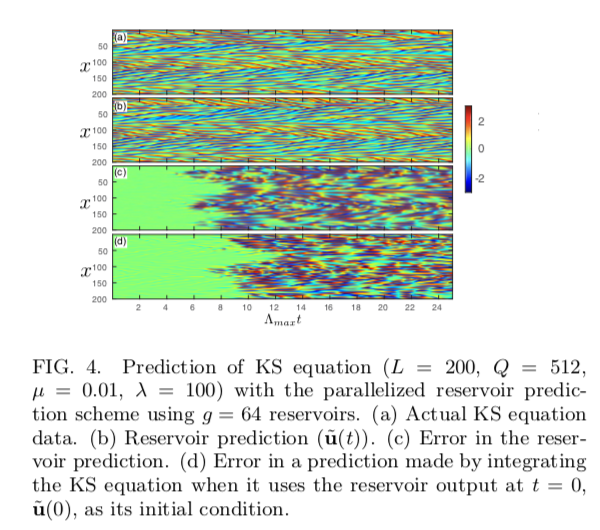
\includegraphics[width = 0.6\textwidth]{figures/pathak_model-free_2018_fig4}}
\end{center}

\vfill
\tiny{\url{https://doi.org/10.1103/PhysRevLett.120.024102}}, about 300 citations

\end{frame}
%%%%%%%%%%%%%%%%%%%%%%%%%%%%%%%%%%%%%%%
\begin{frame}

My 3 takeaways:
\begin{itemize}
\item Deterministic systems can be unpredictable 
\pause
\item Sensitive dependence on initial conditions seems like a formal way to show unpredictability, but it seems different from our other measures of predictability and unpredictability
\pause
\item It now seems hard to imagine any prediction without a time-window attached to it (e.g., a 3-day forecast or a 5-day forecast)
\end{itemize}

\end{frame}
%%%%%%%%%%%%%%%%%%%%%%%%%%
\frame{\titlepage}


\end{document}
